
\chapter{Robot-Camera Calibration}
\label{chap:robot}
This section presents the theory as well as each individual step for estimating the pose of the camera relative to the robot base frame, the problem to be solved is an extrinsic camera calibration (also known as a robot-camera calibration or Eye-to-hand calibration), but an intrinsic camera calibration needs to be solved a priori. The robot-camera calibration is a fundamental part of the subsequent use in the next chapter of this thesis. The extrinsic camera calibration methods generally require the position of the camera frame relative to a calibration target frame to be known. Therefore, the proposed method to solve the robot-camera calibration task for this thesis is based on tracking a calibration target (standard checkerboard calibration grid) attached to the end-effector of the robot with known forward kinematics as seen in the  Figure \ref{fig:system0}. 


\section{Camera Calibration}

Camera calibration is the process of estimating intrinsic and extrinsic parameters. The intrinsic parameters deal with the camera's internal characteristics, such as its focal distance, distortion, and image centre. The extrinsic parameters represent the position and orientation relative to the calibration target. In this thesis, the estimation of intrinsic and extrinsic parameters are treated separately as described above.

\subsection{Intrinsic Calibration}
The choice of camera model influences the final calibration results, so the first step is to select an appropriate camera model. In this thesis, the pinhole camera model \ref{pinhole} is used. It describes the mathematical relationship between the coordinates of a point in three-dimensional space and its projection onto the image plane of an ideal camera. 

Existing algorithms included in the OpenCV library is available for checkerboard detection based on pinhole model and introduces the radial distortion and tangential distortion. The calibration based on openCV is based on the method proposed by Zhang \cite{camCalib}. In addition to that, the $camera\textunderscore calibration$ ROS package \cite{camCalibRos}  based on the same method proposed by Zhang is taken into account for estimating the intrinsic parameter of the camera.
The technique proposed by Zhang only requires the camera to observe a calibration target shown at few (at least two) different orientations. 

\begin{figure}[!h]
\begin{center}
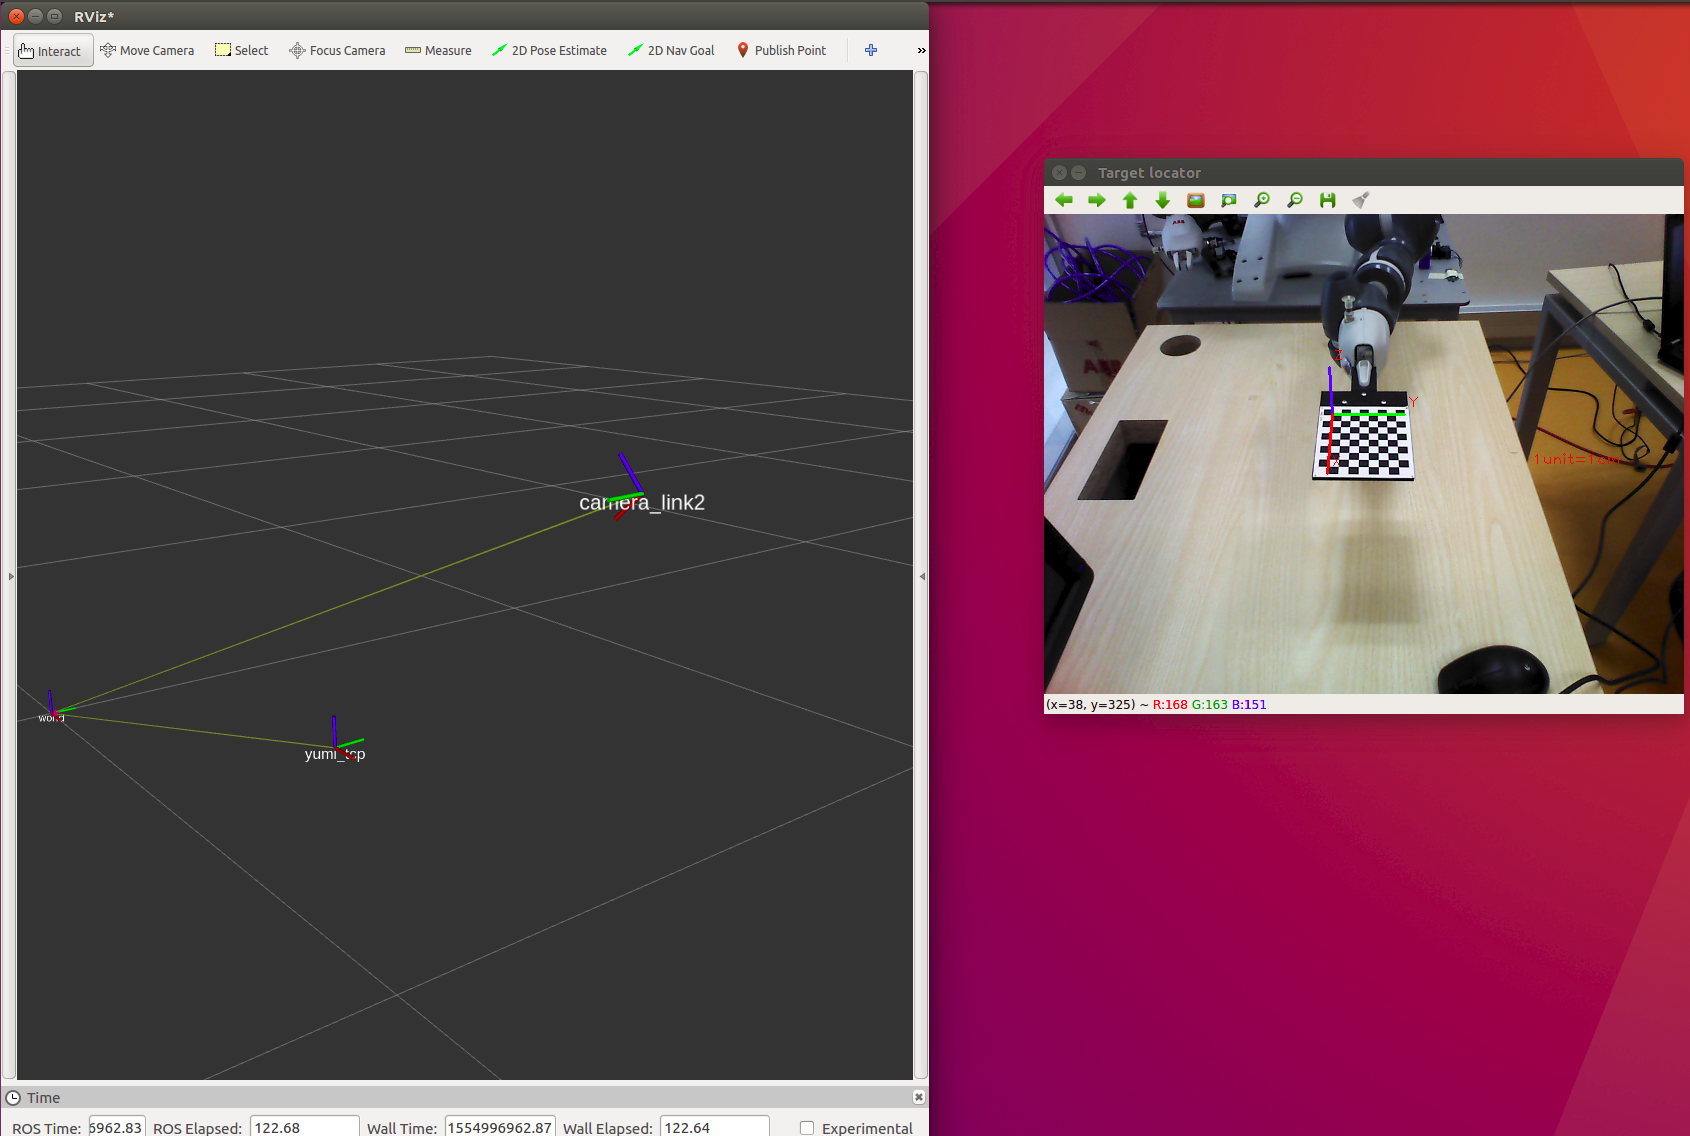
\includegraphics[width=3in]{figures03/rviz1.png}
\caption{Overview of the intrinsic calibration based on industrial calibration (ROS package)}%\cite{temp2}}
\label{fig:rosCAL}
\end{center}
\end{figure}

\begin{figure}[!h]
\begin{center}
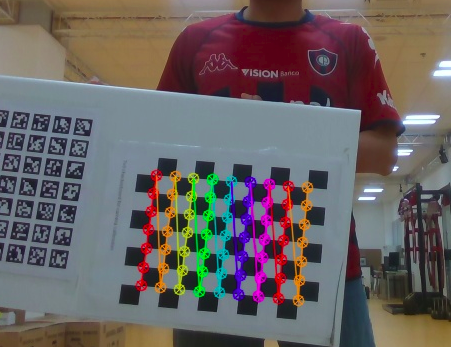
\includegraphics[width=3in]{figures03/openCV1.png}
\caption{Overview of the intrinsic calibration based on industrial calibration (ROS package)}%\cite{temp2}}
\label{fig:rosCAL}
\end{center}
\end{figure}









\begin{figure}[!h]
\begin{center}
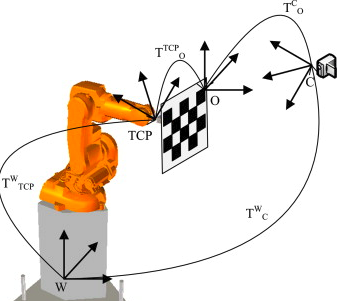
\includegraphics[width=3in]{figures03/system1.png}
\caption{Overview of the camera pose estimation system. The system estimates  the pose of the camera frame relative to the world frame(also known as robot base frame). Image from \cite{autCAL}.}
\label{fig:system0}
\end{center}
\end{figure}





\begin{figure}[!h]
\begin{center}
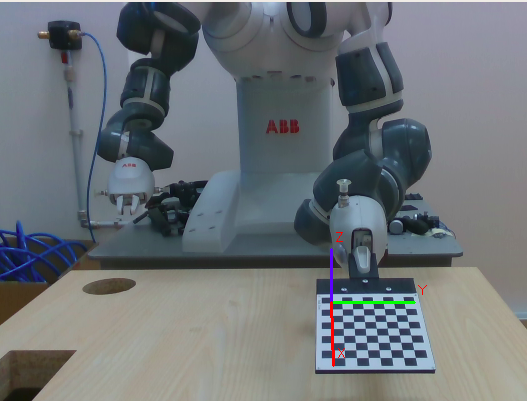
\includegraphics[width=3in]{figures03/robotcamera1.png}
\caption{Overview of the setup and what is being estimated}%\cite{temp2}}
\label{fig:pipeline}
\end{center}
\end{figure}









\begin{figure}[!h]
\begin{center}
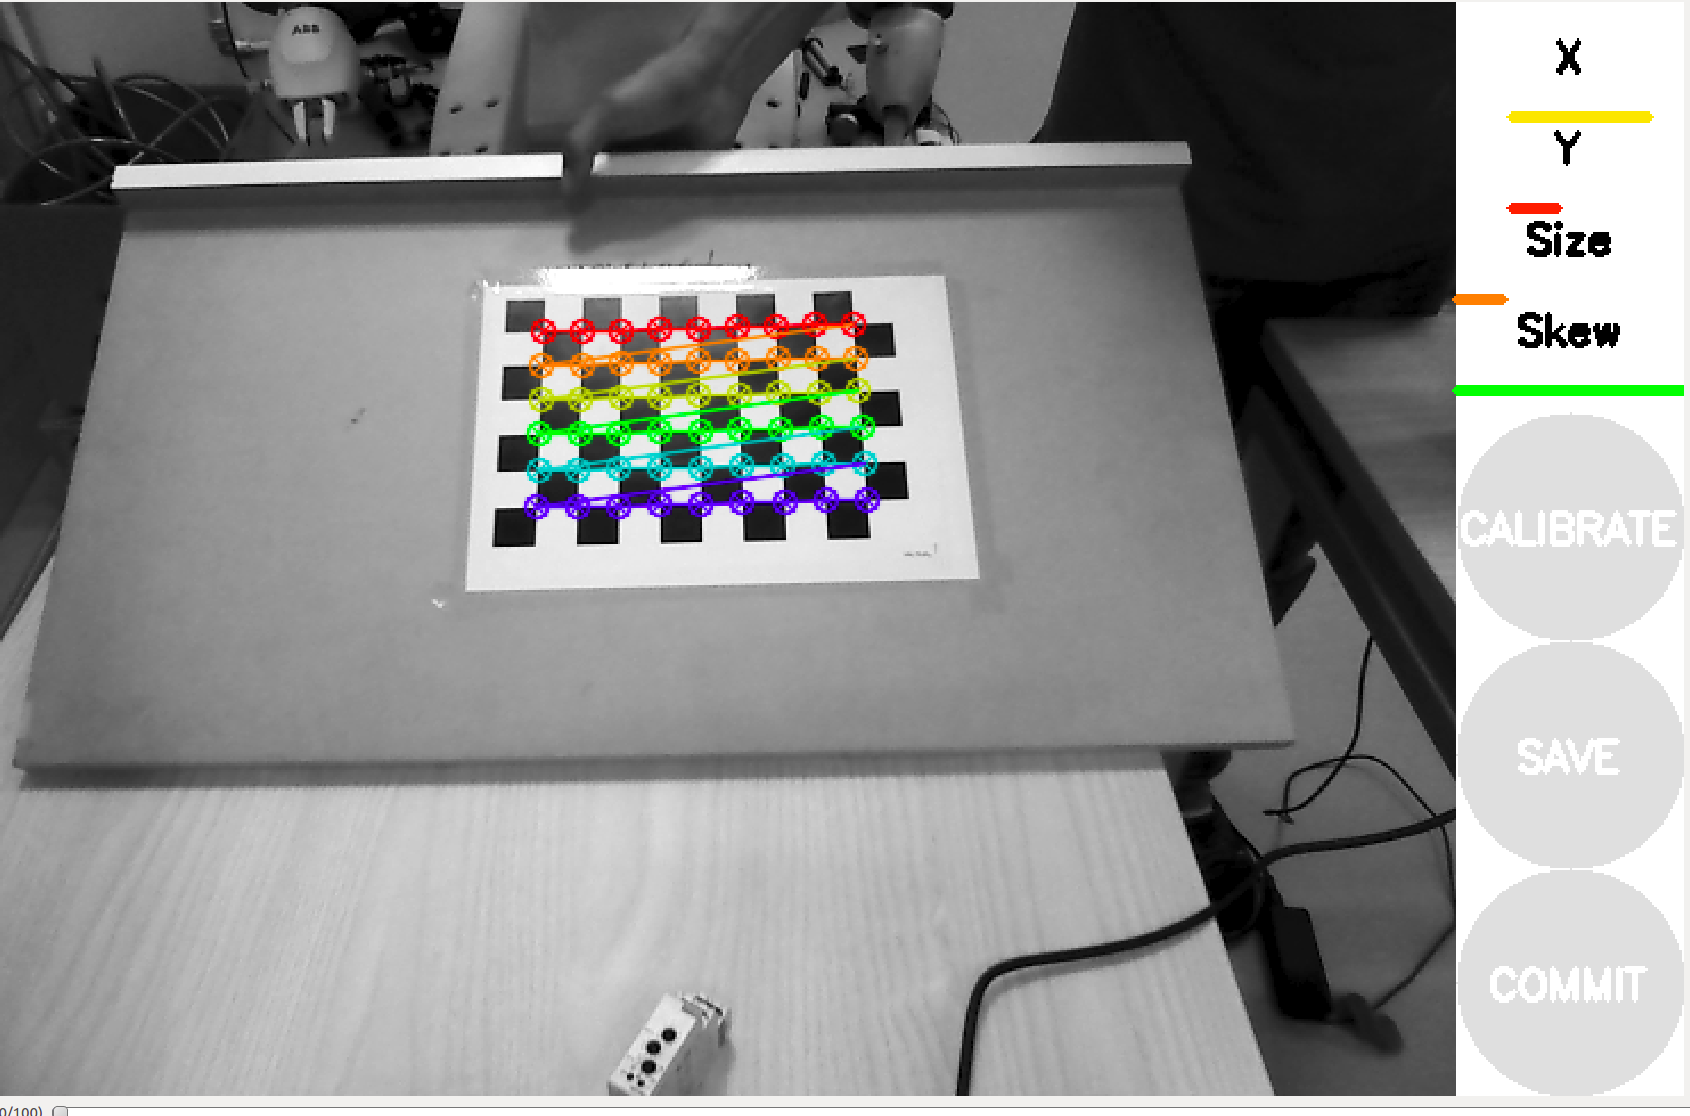
\includegraphics[width=3in]{figures03/intros.png}
\caption{Overview of the intrinsic calibration based on industrial calibration (ROS package)}%\cite{temp2}}
\label{fig:pipeline}
\end{center}
\end{figure}


\begin{figure}[!h]
\begin{center}
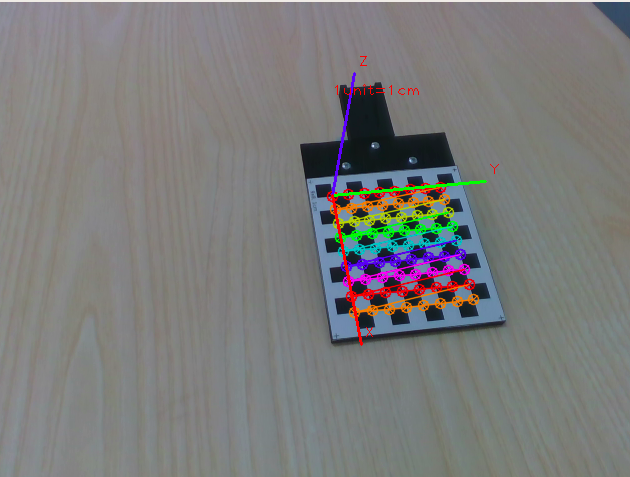
\includegraphics[width=3in]{figures03/calibrationtarget1.png}
\caption{Checkerboard Calibration Target}%\cite{temp2}}
\label{fig:pipeline}
\end{center}
\end{figure}












\iffalse

Camera calibration procedure is performed to obtain the intrinsic and extrinsic camera parameters.The intrinsic parameters are used for obtaining the relative position of the object according to the frame fixed with camera. This procedure is performed only once. The extrinsic parameters are the pose (translation and rotation) of the camera frame with respect to the robot-base frame, this procedure needs to be repeated each time the position of the camera changed with respect to the robot-base frame. 


The robot-camera calibration is based on a checkerboard calibration target attached rigidly to the end-effector of the robot. The position of the calibration target in the end-effector frame is estimated according to the design of the calibration plate in the FreeCAD software, and the pose between the camera frame and the robot base frame is calculated by the Eq. , for convinience of faster calculation, we use the tf-ROS package. The overview of the estimated parameters is presented in Figure. \ref{fig:rviz1} 



industrial calibration OpenCV 2.3 library are used. For cameras position calibration,method presented by Motai and Kosaka[13]has been adopted andimplemented
Although not being the main focus of this project, robot-camera calibration is an essential part for the subsequent step, recognition and estimation of the position of an object with a camera, the main objective of this master thesis. Therefore, the exact transformation between the base frame of the robot and the camera has to be known. 

\fi




































